\documentclass{article}

\usepackage[hangul]{kotex} %<===> EUC-KR
\usepackage{ifxetex} % 부득이하게 pdflatex을 사용해도 문제가 없도록 함

\ifxetex
%한글 사용 옵션
\RequirePackage{xetexko}
\setmainfont[Ligatures=TeX]{Batang}
\setmainhangulfont[BoldFont=*,BoldFeatures=FakeBold,%
ItalicFont=*,ItalicFeatures=FakeSlant]{Batang}
\disablecjksymbolspacing
\nonfrenchspacing
\else
\fi

\usepackage[T1]{fontenc}
\usepackage{pslatex}
\usepackage[pdftex]{color}  
\usepackage[pdftex]{graphicx}     

\usepackage{titlesec}
\usepackage{verbatim}
\usepackage[title,titletoc]{appendix}
\usepackage{booktabs}
\usepackage{graphicx}
\usepackage{tikz}
\begin{document}


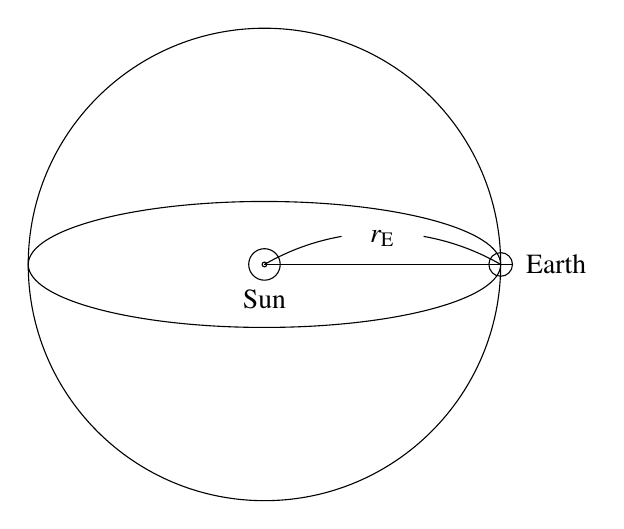
\begin{tikzpicture}[scale = 1, xshift = 1cm]
	\draw (5,2) circle (3cm);
	\draw (5,2) ellipse (3cm and 0.8cm);
	\draw (5,2) circle (0.03cm);
	\draw (5,2) circle (0.2cm) node[below, yshift=-0.2cm] {Sun};
	\draw (8,2) circle (0.15cm) node[right, xshift=0.2cm] {Earth};
	\draw (5,2) -- (8,2) node[above, xshift=-1.5cm, yshift=0.1cm] {$r_{\mathrm{E}}$};
	\draw (5,2) arc (120:100:3cm);
	\draw (8,2) arc (60:80:3cm);
	\draw (7.85,2) -- (8.15,2);
	\draw (8,1.85) -- (8,2.15);
\end{tikzpicture}

\vspace{1cm}
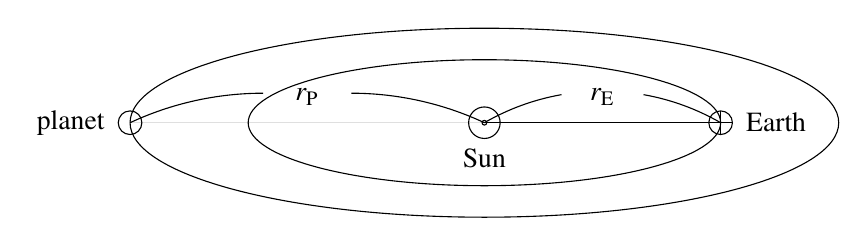
\begin{tikzpicture}[scale = 1, xshift = 1cm]
	\draw (5,2) ellipse (3cm and 0.8cm);
	\draw (5,2) ellipse (4.5cm and 1.2cm);
	\draw (5,2) circle (0.03cm);
	\draw (5,2) circle (0.2cm) node[below, yshift=-0.2cm] {Sun};
	\draw (8,2) circle (0.15cm) node[right, xshift=0.2cm] {Earth};
	\draw (5,2) -- (8,2) node[above, xshift=-1.5cm, yshift=0.1cm] {$r_{\mathrm{E}}$};
	\draw (5,2) arc (120:100:3cm);
	\draw (8,2) arc (60:80:3cm);
	\draw (0.5,2) circle (0.15cm) node[left, xshift=-0.2cm] {planet};
	\fill (5,2) -- (0.5,2) node[above, xshift=2.25cm, yshift=0.1cm] {$r_{\mathrm{P}}$};
	\draw (0.5,2) arc (115:90:4cm);
	\draw (5,2) arc (65:90:4cm);
	\draw (7.85,2) -- (8.15,2);
	\draw (8,1.85) -- (8,2.15);
\end{tikzpicture} 
	
\vspace{1cm}
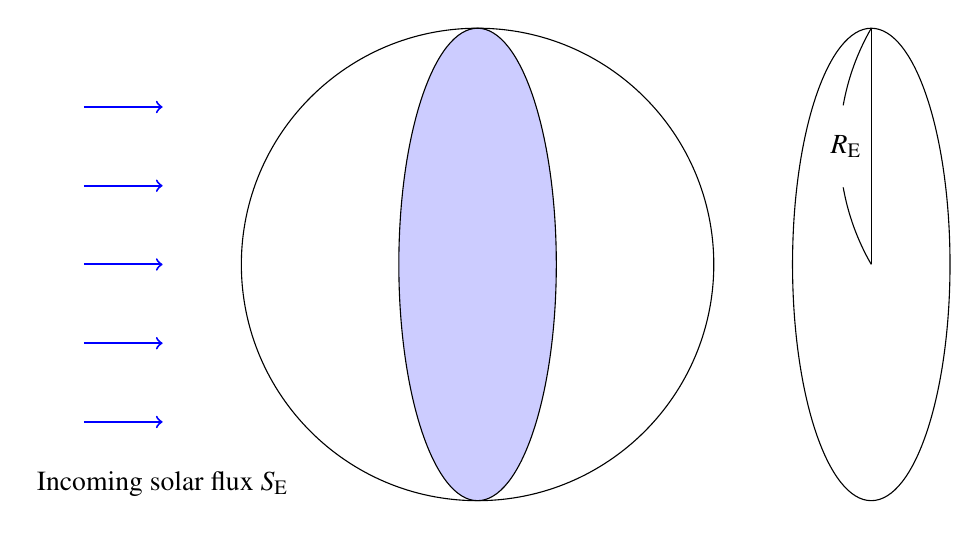
\begin{tikzpicture}[scale = 1, xshift = 1cm]
	\draw [line width=0.25mm, blue] [->] (0,0) -- (1,0) node[black, below, yshift=-0.5cm] {Incoming solar flux $S_{\mathrm{E}}$};
	\draw [line width=0.25mm, blue] [->] (0,1) -- (1,1);
	\draw [line width=0.25mm, blue] [->] (0,2) -- (1,2);
	\draw [line width=0.25mm, blue] [->] (0,3) -- (1,3);
	\draw [line width=0.25mm, blue] [->] (0,4) -- (1,4) ;
	
	\draw (5,2) circle (3cm);
	
	\fill [blue!20!white] (5,2) ellipse (1cm and 3cm) ;
	\draw (5,2) ellipse (1cm and 3cm) ;
	\draw (10,2) ellipse (1cm and 3cm);
	\draw (10,2) -- (10,5) node[left, yshift=-1.5cm] {$R_{\mathrm{E}}$};
	\draw (10,2) arc (210:190:3cm);
	\draw (10,5) arc (150:170:3cm);
\end{tikzpicture}
\end{document}

